\let\negmedspace\undefined
\let\negthickspace\undefined
\documentclass[journal]{IEEEtran}
\usepackage[a5paper, margin=10mm, onecolumn]{geometry}
%\usepackage{lmodern} % Ensure lmodern is loaded for pdflatex
\usepackage{tfrupee} % Include tfrupee package

\setlength{\headheight}{1cm} % Set the height of the header box
\setlength{\headsep}{0mm}     % Set the distance between the header box and the top of the text

\usepackage{gvv-book}
\usepackage{gvv}
\usepackage{cite}
\usepackage{amsmath,amssymb,amsfonts,amsthm}
\usepackage{algorithmic}
\usepackage{graphicx}
\usepackage{textcomp}
\usepackage{xcolor}
\usepackage{txfonts}
\usepackage{listings}
\usepackage{enumitem}
\usepackage{mathtools}
\usepackage{gensymb}
\usepackage{comment}
\usepackage[breaklinks=true]{hyperref}
\usepackage{tkz-euclide} 
\usepackage{listings}
% \usepackage{gvv}                                        
\def\inputGnumericTable{}                                 
\usepackage[latin1]{inputenc}                                
\usepackage{color}                                            
\usepackage{array}                                            
\usepackage{longtable}                                       
\usepackage{calc}                                             
\usepackage{multirow}                                         
\usepackage{hhline}                                           
\usepackage{ifthen}                                           
\usepackage{lscape}
\usepackage{circuitikz}
\tikzstyle{block} = [rectangle, draw, fill=blue!20, 
    text width=4em, text centered, rounded corners, minimum height=3em]
\tikzstyle{sum} = [draw, fill=blue!10, circle, minimum size=1cm, node distance=1.5cm]
\tikzstyle{input} = [coordinate]
\tikzstyle{output} = [coordinate]
\begin{document}

\bibliographystyle{IEEEtran}
\vspace{3cm}

\title{1.10.10}
\author{EE25BTECH11051 - Shreyas Goud Burra}
\maketitle
% \newpage
% \bigskip
{\let\newpage\relax\maketitle}

\renewcommand{\thefigure}{\theenumi}
\renewcommand{\thetable}{\theenumi}
\setlength{\intextsep}{10pt} % Space between text and floats


\numberwithin{equation}{enumi}
\numberwithin{figure}{enumi}
\renewcommand{\thetable}{\theenumi}

\textbf{Question}
The vector in the direction of the vector $\hat{i} - 2\hat{j} + 2\hat{k}$ that has magnitude 9 is
\begin{enumerate}[label=(\alph*)]
    \item $\hat{i}-2\hat{j}+2\hat{k}$
    \item $\hat{i}-2\hat{j}$
    \item $3(\hat{i}-2\hat{j}+2\hat{k})$
    \item $9(\hat{i}-2\hat{j}+2\hat{k})$
\end{enumerate}

\solution \\

Let us solve the given equation theoretically and then verify the solution computationally.

Let us assume the given vector to be vector \textbf{A}

\begin{align}
    \textbf{A} = \myvec{1 \\ -2 \\ 2}
    \label{4.1}
\end{align}

First we find the unit vector in the direction of the given vector.\\
This is given by:

\begin{align}
    \hat{\textbf{A}} = \frac{\textbf{A}}{\norm{\textbf{A}}}
    \label{4.2}
\end{align}

Here the magnitude(norm) of the vector \textbf{A} is given by

\begin{align}
    \textbf{A}^T\textbf{A} = \norm{\textbf{A}}^2
    \label{4.3}
    \implies \myvec{1 & -2 & 2} \myvec{1 \\ -2 \\ 2} = 9
\end{align}

\begin{align}
    \implies \norm{\textbf{A}} = 3
    \label{4.4}
\end{align}

From \ref{4.4}, this gives us

\begin{align}
    \hat{\textbf{A}} = \frac{\textbf{A}}{\norm{\textbf{A}}} = \frac{1}{3} \myvec{1 \\ -2 \\ 2}
    \label{4.5}
\end{align}

\newpage

From \ref{4.5}, the vector of magnitude $9$ along this direction is given by

\begin{align}
    9\hat{\textbf{A}} = 9 \times \frac{1}{3}\myvec{1 \\ -2 \\ 2}
    \label{4.6}
\end{align}

\begin{align}
    \implies 3\myvec{1 \\ -2 \\ 2} = 3(\hat{i}-2\hat{j}+2\hat{k})
    \label{4.7}
\end{align}

Therefore the required vector is $3(\hat{i}-2\hat{j}+2\hat{k})$. This is option (b).\\

We get the same result by plotting a graph for the following.
\begin{figure}[H]
    \centering
    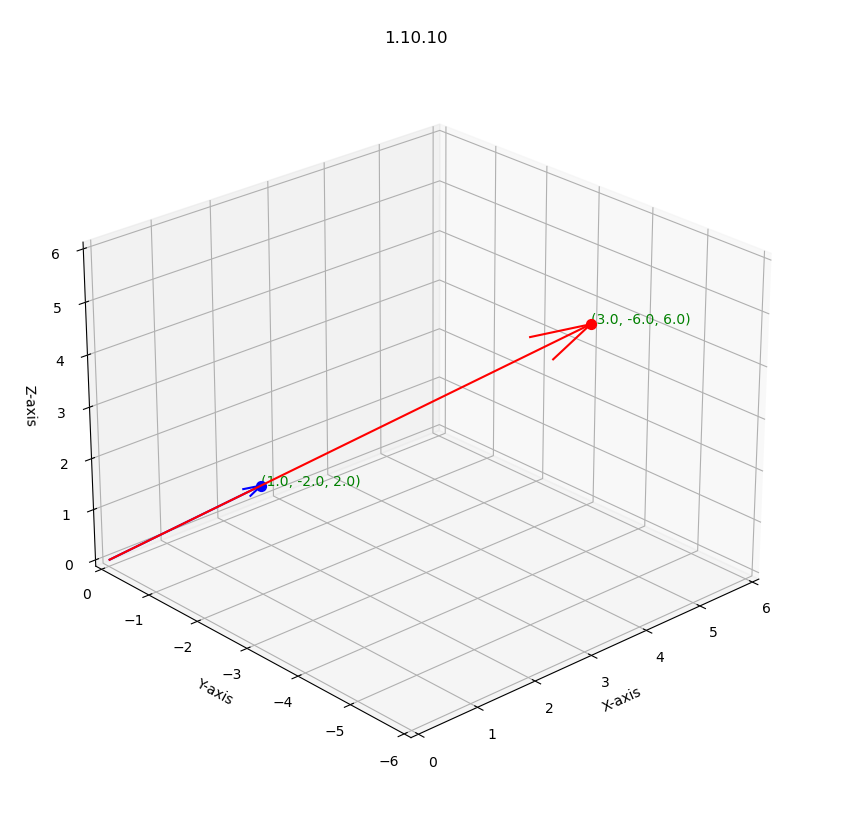
\includegraphics[width=0.8\columnwidth]{figs/fig1.png}
    \caption{3D Plot}
    \label{3D Plot}
\end{figure}


\end{document}
